\section{Software}
\label{Sec:software}
Para que a aplicação Web possa receber os dados de consumo enviados pelo Módulo Coordenador, é necessário haver uma estrutura de rotas, métodos para lidar com objetos de classes, controladores e páginas de exibição para interagir com o usuário. Para isso, foi escolhida a arquitetura MVC, e um framework que consegue lidar com tal arquitetura. E para tornar a aplicação disponível para o acesso remoto através de smartphones, tablets e notebooks, optou-se por utilizar serviços de nuvem. 

\subsection{Tecnologia}

A seguir são apresentadas as tecnologias utilizadas para a implementação da aplicação Web.

\subsubsection{Django e Python}

O framework Django \cite{django_framework_site} foi utilizado devido ao uso da linguagem python, que é uma linguagem limpa, de fácil utilização e com ampla disponibilidade de bibliotecas gratuitas e de fóruns para auxílio na implementação. Uma das vantagens do python nesse caso é a compatibilidade, pois o hardware foi construído com intenção de aprendizado através da linguagem de programação python \cite{raspberry_pi_site}(``pi'' em ``raspberry pi'' vem de ``python''). Outra vantagem é a experiência dos integrantes do grupo quanto ao manuseio do framework, o que agilizou o desenvolvimento. Outra vantagem é a possibilidade de utilizar, se necessário, o próprio raspberry como servidor da aplicação, bastando instalar as bibliotecas das dependências do Django.

O Django utiliza a arquitetura MVC. Os Models no Django contém os campos e os métodos dos objetos sendo utilizados. Todos as classes de Models herdam métodos e atributos da classe pré-existente Model do Django. Geralmente, cada Model é mapeado para uma tabela no banco de dados.

As Views (na arquitetura MVC) são chamadas Templates no Django. Elas são páginas no formato HTML que podem conter trechos de código em python para mostrar conteúdo do Context. Context é uma estrutura de chave-valor que provê o conteúdo a ser utilizado na página.

Os Controllers são chamados Views. O Django provê os chamados Base Views, que são classes que auxiliam a criação de Controllers. Podem ser utilizados diretamente, sobrescrevendo seus atributos e métodos, ou herdando estes para classes customizadas. Há três Base Views: 
\begin{description}
	\item[View:] É a classe a partir da qual se herdam todas as outras classes de Controllers.
	\item[TemplateView:] Renderiza um Template com um Context.
	\item[RedirectView:] Redireciona para uma dada URL.
\end{description} 

Outros Controllers pré-existentes são os Generic Display Views, que são Controllers genéricos utilizados normalmente para exibir dados de Models:
\begin{description}
	\item[DetailView:] Exibe detalhes um objeto.
	\item[ListView:] Exibe uma lista de objetos.
\end{description}

Há Controllers utilizados para edição de conteúdo, que são os Generic Editing Views:
\begin{description}
	\item[FormView:] Exibe um formulário e realiza validação e redirecionamento caso não haja erros.
	\item[CreateView:] Exibe um formulário para criação de objetos. Caso o formulário seja submetido e não haja erros na validação, cria o objeto.
	\item[UpdateView:] Exibe um formulário para edição de objetos. Caso o formulário seja submetido e não haja erros na validação, salva o objeto.
	\item[DeleteView:] Exibe uma página com uma caixa de confirmação para deletar um objeto.
\end{description}

\subsubsection{Heroku}

Heroku é uma plataforma em nuvem que fornece múltiplos serviços para dar suporte a uma aplicação web. É possível hospedar aplicações em linguagens como Node, Ruby, Java, PHP, Python, Go, Scala, ou Clojure, e o Heroku a manterá no ar sem a necessidade da intervenção do desenvolvedor. Esse serviço, diferente de opções de outros serviços de nuvem como o da Amazon, se encarrega em configurar o ambiente de execução da aplicação, o que agiliza o processo de colocar a aplicação em produção.

Heroku utiliza os chamados dynos, que representam máquinas/computadores que executam comandos. Cada tipo de dyno possui a sua limitação de memória RAM, fração de CPU, se é dedicada ou não e a velocidade do processamento, que refletem nos custos de aquisição dos serviços, porém, existe a opção gratuita que permite colocar uma aplicação em produção com um processamento suficiente para atender tráfegos pequenos. Nos planos pagos, o sistema é escalável (pode-se alterar o limite do número de processos em execução na máquina do sistema, memória RAM, entre outros) para atender a momentos de tráfego mais intenso.\cite{heroku}

Durante a fase de teste do sistema em questão é utilizado o plano gratuito do Heroku.

\subsection{Funções do Sistema}

A aplicação Web possui tem como objetivo mostrar os dados de consumo para o usuário, mas a aplicação deve possuir outras funções para alcançar o objetivo. Uma delas é criar uma conta. Para que o usuário possa manter seus dados confidenciais, a aplicação permite autenticação através de senha e nome de usuário. Equipamentos são  representados dentro do sistema, para que cada consumo possa se associar a um equipamento, e para isso, é necessário que o usuário gerencie os seus equipamentos. Os sensores também são representados dentro do sistema, pois um usuário tem a opção de alocar o sensor de um equipamento para outro, caso deseje. O Módulo Coordenador cria os consumos dentro do sistema, enquanto o usuário visualiza, importa e exporta os consumos. Para que a conversão do consumo em unidades monetárias seja possível, o usuário deve atualizar as taxas da AES dentro do sistema. E para fazer a associação entre um sensor e um equipamento e atualizar suas informações de renda, o usuário deve configurar o sistema. A partir dessas informações foi criada a seguinte lista de funções para a aplicação:

\begin{description}
	\item[Gerenciar contas:] O usuário pode fazer cadastro/alteração de conta e autenticação.
	\item[Gerenciar equipamentos:] O usuário pode fazer a criação, edição e remoção de equipamentos.
	\item[Gerenciar sensores:] Os módulos sensores são auto-detectados, e o usuário pode editá-los ou removê-los.
	\item[Gerenciar metas:] O usuário pode criar, editar e remover metas mensais.
	\item[Gerenciar consumo:] O Módulo Coordenador envia consumos para o sistema. O usuário pode visualizar os consumos através de gráficos. Além disso o usuário pode importar ou exportar dados de consumo.
	\item[Atualizar taxas da AES:] O usuário pode atualizar as taxas de energia utilizadas para cálculo do custo do consumo.
	\item[Configurar sistema:] O usuário pode associar os sensores aos equipamentos e escolher um tipo de renda.
\end{description}

\subsection{Atores}

A partir da descrição dos casos de uso (apêndice \ref{apendice_caso_uso}), dois atores foram identificados: o usuário e o módulo coordenador, que são as entidades externas que interagem com o sistema.

\begin{description}
	\item[usuário:] Como o sistema vai ser utilizado apenas pelo(s) responsável(is) pela residência, há apenas um tipo de usuário, que é o usuário comum.
    \item[módulo coordenador:] É o componente de hardware que enviará informações de consumo para o sistema
\end{description}

%
\subsection{Classes e atributos}

A partir dos casos de uso foi possível a identificação das classes dentro do sistema: Equipment, Consumption, Sensor, AESRate, Goal, User. Essas classes e suas relações estão representadas pelo diagrama de classes na figura \ref{fig:diagrama-classes}.

\begin{figure}[H]
\begin{center}
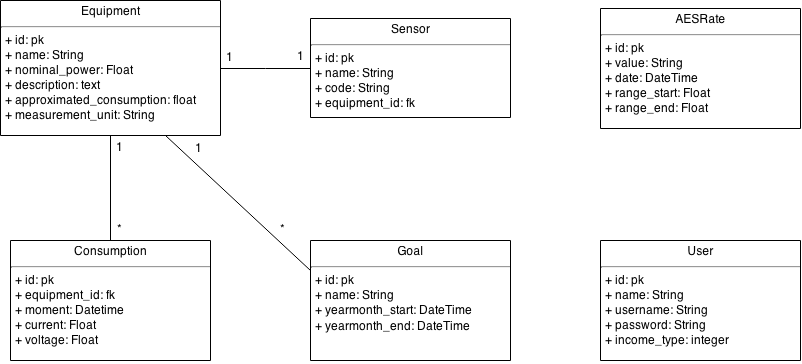
\includegraphics[width=1\textwidth]{figuras/diagrama_classes.png}
\caption{\label{fig:diagrama-classes} Diagrama de Classes}
\end{center}
\end{figure}

A descrição das classes está no apêndice \ref{apendice_classes}